\chapter{ Local Features - Harris Corner Detection}

\noindent
En visión por computadora, para resolver problemas como el emparejamiento de imágenes o el rastreo de objetos, no analizamos la imagen global de golpe. En su lugar, buscamos \textbf{características locales} (puntos de interés) que sean distintivos, repetibles y robustos a transformaciones. \\ \\
\noindent
El objetivo de todo este ecosistema (Harris + Feature Matching + RANSAC) no es tomar dos fotos globales y decir: ``A ver, ¿se parecen en un 80\%?''. No estamos haciendo una comparación global de imágenes. Su verdadero propósito es localizar elementos idénticos dentro de ellas para poder alinearlas, transformarlas y unirlas geométricamente (Image Alignment \& Stitching).\\ \\
\noindent
El flujo de trabajo se divide en dos componentes críticos que debemos diferenciar perfectamente:
\begin{enumerate}
    \item \textbf{Detector de Características (Feature Detector):} algoritmo encargado de buscar e identificar de forma precisa \textit{dónde} están los puntos de interés en la imagen (coordenadas $(x,y)$), como esquinas o manchas.
    \item \textbf{Descriptor de Características (Feature Descriptor):} un vector matemático que codifica la apariencia visual de la vecindad o parche que rodea al punto detectado. Convierte la información visual en una firma matemática única para poder compararla con descriptores de otras imágenes.
\end{enumerate}
\begin{definicion}
    Un \tbf{feature descriptor} es un vector matemático de números (una lista ordenada de valores continuos) que codifica de forma compacta y única cómo se ve visualmente la región o parche de la imagen que rodea a esa esquina.  En lugar de guardar solo el píxel central de la esquina, el descriptor analiza el vecindario (por ejemplo, una ventana de $16 \times 16$ píxeles alrededor de la esquina). A esa ventana le extrae información matemática clave, como por ejemplo:  
    \begin{itemize}
        \item \tbf{Dirección}: dirección hacia la que apuntan los gradientes de brillo (si hay cambios hacia arriba, abajo, diagonales).
        \item \tbf{Textura}: la distribución de las texturas locales.
        \item \tbf{Contraste}: el contraste o las intensidades relativas.
    \end{itemize}
    Toda esa estructura visual se ``aplana'' y se transforma en un vector de números (un vector de características).
\end{definicion}

\section{Harris Corner Detector}
\noindent
\begin{definicion}
    Una \tbf{esquina} (o keypoint) se define idealmente como una región de la imagen donde la intensidad del brillo cambia drásticamente en \underline{todas las direcciones}. Cuando hablamos de todas las direcciones, nos referimos a dos fuerzas de cambio ortogonales (perpendiculares) e independientes que rellenan todo el espacio bidimensional.\\ 
\end{definicion}

\observacion{
    Uno de primeras puede pensar que para detectar una esquina, basta con analizar los cambios de intensidad en horizontal y vertical. Sin embargo, esto no es suficiente. Para entenderlo, imaginemos una línea diagonal perfectamente inclinada a $45^\circ$. Si nos movemos un píxel hacia la derecha (horizontal), el brillo cambia. Si nos movemos un píxel hacia abajo (vertical), el brillo también cambia. Alguien podría pensar: ``¡Ostras! Cambia en horizontal y cambia en vertical, ¡entonces es una esquina!''. \tbf{Falso}. Si en esa misma línea diagonal intentamos moverte en la dirección de la propia diagonal (combinando avanzar a la derecha y avanzar hacia abajo a la vez), verás que el brillo no cambia en absoluto, porque te estás deslizando a lo largo de la línea. Por lo tanto, no es una esquina, es un borde inclinado (Edge). Sus cambios horizontales y verticales estaban ``atados'' por la misma pendiente. \\
}

\begin{observacion}
    Cuando hablamos de esquina, no tiene porque ser una esquina geométrica perfecta, puede ser cualquier punto que tenga un cambio de intensidad fuerte en todas las direcciones, por lo que muchas veces se nombrará como \textbf{punto de interés} o \textbf{keypoint} para evitar confusiones. En la práctica, lo que el detector de Harris busca es precisamente eso: puntos de interés que tengan una estructura local rica en información visual, lo que los hace ideales para tareas de emparejamiento y reconocimiento.\\
\end{observacion}

\noindent
Para entonces poder analizar con exactitud una esquina, seguiremos el siguiente proceso y nos centraremos en el \tbf{tensor de estructura} (structure tensor) que es la base matemática del detector de Harris. \\

\noindent
Primero, analizamos cómo cambia la intensidad al desplazar una ventana local $(u,v)$ una pequeña distancia $(x,y)$. La función de suma de diferencias al cuadrado ($E$) se define como:
$$E(x,y) = \sum_{u,v} w(u,v) \left[ I(u+x, v+y) - I(u,v) \right]^2$$
donde $w(u,v)$ es una función de ventana (uniforme o Gaussiana). Aplicando una aproximación por \tbf{Serie de Taylor} de primer orden para pequeñas traslaciones:
$$I(u+x, v+y) \approx I(u,v) + I_x x + I_y y$$
y sustituyendo esto en la ecuación original, llegamos a la forma cuadrática fundamental
$$E(x,y) \approx \begin{bmatrix} x & y \end{bmatrix} H\begin{bmatrix} x \\ y \end{bmatrix}$$

\begin{notacion}
    Aquí tenemos dos términos importante tener claros:
    \begin{itemize}
        \item $I_x$ (\tbf{Gradiente Horizontal}): Mide cuánto cambia el brillo de la imagen cuando te mueves de izquierda a derecha (horizontalmente, a lo largo del eje $X$).
        \item $I_y$ (\tbf{Gradiente Vertical}): Mide cuánto cambia el brillo de la imagen cuando te mueves de arriba a abajo (verticalmente, a lo largo del eje $Y$).
    \end{itemize}
\end{notacion}

\subsection{Structure Tensor}
\begin{definicion}
    La matriz $H$ se conoce como el \textbf{Tensor de Estructura} (o matriz de covarianza de gradientes) y condensa la distribución de los gradientes locales en la ventana:
    $$H = \sum_{u,v} w(u,v) \begin{bmatrix} I_x^2 & I_x I_y \\ I_x I_y & I_y^2 \end{bmatrix} = \begin{bmatrix} \langle I_x^2 \rangle & \langle I_x I_y \rangle \\ \langle I_x I_y \rangle & \langle I_y^2 \rangle \end{bmatrix}$$
\end{definicion}

\noindent
Las propiedades geométricas de la vecindad quedan codificadas por los \tbf{autovalores} ($\lambda_1, \lambda_2$) de la matriz $H$:
\begin{itemize}
    \item \textbf{Región Plana (Flat):} $\lambda_1 \approx 0$ y $\lambda_2 \approx 0$ (no hay cambios de intensidad en ninguna dirección).
    \item \textbf{Edge:} un autovalor es grande y el otro es pequeño ($\lambda_1 \gg 0, \lambda_2 \approx 0$). Solo hay cambio de intensidad perpendicular al borde.
    \item \textbf{Corner:} ambos autovalores son grandes ($\lambda_1 \gg 0$ y $\lambda_2 \gg 0$). Hay cambios fuertes en todas las direcciones.
\end{itemize}

\subsection{Función de Respuesta de Esquina ($R$)}
\noindent
Calcular los autovalores exactos para cada píxel es computacionalmente costoso. Harris y Stephens propusieron una alternativa elegante utilizando el determinante y la traza de la matriz $H$:
$$R = \det(H) - k \cdot (\text{traza}(H))^2$$
Donde:
\begin{itemize}
    \item $\det(H) = \lambda_1 \lambda_2 = (I_x^2)(I_y^2) - (I_x I_y)^2$
    \item $\text{traza}(H) = \lambda_1 + \lambda_2 = I_x^2 + I_y^2$
    \item $k$ es una constante empírica (típicamente $k \in [0.04, 0.06]$).
\end{itemize}
\subsubsection{Clasificación según la respuesta $R$}
\begin{itemize}
    \item Si $R > 0 \longrightarrow$ Es una \tbf{esquina} (Ambos autovalores dominan).
    \item Si $R < 0 \longrightarrow$ Es un \tbf{borde} ($\det(H)$ es pequeño frente a la traza al cuadrado).
    \item Si $|R|$ es pequeño $\longrightarrow$ Es una \tbf{región plana}.
\end{itemize}

\subsection{Algoritmo de Harris}
\noindent
Para programar o evaluar el detector de Harris, se siguen estos pasos ordenados:
\begin{enumerate}
    \item \textbf{Compute gradients:} calcular las derivadas espaciales de la imagen $I_x$ e $I_y$ (por ejemplo, usando filtros de Sobel).
    \item \textbf{Build structure tensor:} calcular los productos de gradientes píxel a píxel: $I_x^2$, $I_y^2$, e $I_x I_y$.
    \item \textbf{Apply Window Smoothing (suavizado de la ventana):} filtrar las imágenes de los componentes anteriores con una Gaussiana $w(u,v)$ para obtener los promedios locales $\langle I_x^2 \rangle$, $\langle I_y^2 \rangle$ y $\langle I_x I_y \rangle$.
    \item \textbf{Compute corner response ($R$):} evaluar la fórmula de Harris para cada píxel, de manera que se tiene una matriz de valores $R$ de igual tamaño que la imágen original que indica la fuerza de la esquina en cada ubicación.
    \item \textbf{Threshold corners} :filtrar los píxeles manteniendo solo aquellos donde $R$ supere un umbral predefinido $T_{h\_harris}$ lo que provocará que una zona (por ejemplo, alrededor del pico de una mesa) se detecte como una esquina fuerte.
    \item \tbf{Non-Maximum Suppression}: se realizará una búsqueda local para conservar únicamente los picos locales (máximos locales), evitando que una sola esquina genere múltiples detecciones agrupadas, y podamos obtener un conjunto limpio de puntos de interés sin redundancias. Lo que se hace es lo siguiente:
    \begin{enumerate}
        \item Se define un vecindario local, es decir, una ventana de tamaño fijo centrada en el píxel actual.
        \item Se compara el valor de $R$ del píxel central con los valores de $R$ de todos los píxeles vecinos dentro de esa ventana.
        \item Si el píxel central tiene el valor de $R$ más alto de todo su vecindario, se conserva como una esquina válida. Si cualquier vecino tiene un valor de $R$ estrictamente mayor que el píxel central, entonces el píxel central se descarta (se le asigna un valor de 0), ya que no es un pico local.
    \end{enumerate}
\end{enumerate}

\subsection{Robustez y Limitaciones de Harris}
\begin{itemize}
    \item \textbf{Robusto a la Rotación (Rotation invariant):} la matriz $M$ rota de forma solidaria con la imagen, pero sus autovalores permanecen matemáticamente \textbf{invariantes}. Por ende, una esquina sigue detectándose como esquina aunque giremos la foto.
    \item \textbf{Robusto a cambios de intensidad (Intensity shifts):} al basarse estrictamente en derivadas (gradientes), añadir una constante de brillo a la imagen no altera el resultado ($I_x$ sigue siendo igual). Es parcialmente robusto a cambios afines de iluminación.
    \item \textbf{NO es invariante a la Escala (Not scale invariant):} \textit{¡Pregunta clave de examen!} Si haces un zoom gigante a una esquina, lo que a escala pequeña parecía un punto afilado pasa a verse a escala macroscópica como un borde suave y plano dentro de la pequeña ventana del filtro. El detector de Harris estándar \underline{falla si hay cambios drásticos de escala}.
\end{itemize}

\section{Feature Matching}
\noindent
Una vez que hemos detectado los puntos e indexado sus descriptores vectoriales de apariencia entre dos imágenes distintas, debemos cruzarlos para encontrar correspondencias. La idea aqui, es poder encontrar puntos que se vean igual en ambas fotos, aunque estén tomadas desde ángulos o condiciones de iluminación diferentes. Para esto, existen varias estrategias de matching que se basan en comparar la similitud entre los descriptores de las esquinas detectadas en ambas imágenes.

\subsection{Estrategias de Matching}
\begin{itemize}
    \item \textbf{Descriptor distance comparison:} medimos la similitud calculando la distancia euclídea ($L_2$) o la distancia de Manhattan ($L_1$) entre los vectores de características.
    \item \textbf{Nearest Neighbor Matching (NN):} para un punto de interés en la Imagen A, buscamos el punto en la Imagen B cuyo descriptor tenga la distancia mínima absoluta.
    \item \textbf{Ratio Test (Lowe idea):} el vecino más cercano puro puede fallar si hay texturas repetitivas. Para asegurar que el match es ambiguo o sólido, calculamos la razón entre la distancia del primer vecino más cercano ($d_1$) y la distancia del segundo vecino más cercano ($d_2$):
    $$\text{Ratio} = \frac{d_1}{d_2}$$
    Si esta razón es menor que un umbral estricto (ej. $\le 0.8$), aceptamos el match. Si se acerca a 1, significa que el punto se parece a múltiples zonas de la imagen (ambigüedad), por lo que se descarta.
\end{itemize}

\section{Algoritmo RANSAC}

\noindent
A pesar de aplicar el \underline{ratio test}, en el mundo real siempre aparecen \tbf{outliers}, por lo que para estimar un modelo geométrico válido (como una homografía o matriz fundamental) ignorando los outliers, se utiliza el algoritmo \tbf{RANSAC (RANdom Sample Consensus)}. \\

\begin{definicion}
    Un \tbf{outlier} es un punto de correspondencia que no sigue el modelo geométrico dominante que estamos tratando de estimar. En otras palabras, es un \underline{match erróneo} causado por oclusiones, ruido o cambios de perspectiva.
\end{definicion}

\subsection{Algoritmo RANSAC}
\noindent
RANSAC es un enfoque iterativo basado en la siguiente filosofía de muestreo aleatorio:
\begin{enumerate}
    \item \textbf{Randomly sample:} seleccionar de forma completamente aleatoria un subconjunto mínimo de correspondencias necesarias para calcular el modelo matemático (por ejemplo, 4 pares de puntos para una Homografía). Ese subconjunto se toma de nuestro conjunto de \tbf{esquinas} (o keypoints) emparejadas entre las dos imágenes, usando feature matching.
    \item \textbf{Estimate model:} calcular los parámetros del modelo geométrico provisional basándose únicamente en ese subconjunto mínimo.
    \item \textbf{Count inliers:} evaluar el modelo calculado con el resto de todas las correspondencias de la imagen. Contar cuántos puntos se adaptan al modelo dentro de un umbral de tolerancia de error (estos puntos válidos se llaman \textbf{Inliers}), de la siguiente manera:
    \begin{itemize}
        \item Tomamos un punto $p_i$ de la primera imagen y lo proyectamos usando el modelo provisional calculado ($H p_i$).
        \item Medimos la distancia euclídea en píxeles entre dónde cayó esa proyección teórica y dónde está el punto real emparejado en la segunda imagen ($p'_i$).
        \item Si esa distancia es menor que un umbral de tolerancia $\varepsilon$ (un margen de error pequeño, por ejemplo, 1 o 2 píxeles), el punto se considera un Inlier (un voto a favor del modelo). Si la distancia es mayor, se ignora por ser un outlier.
    \end{itemize}

    \item \textbf{Repeat:} repetir este proceso de muestreo (los 3 pasos anteriores), estimación y conteo de inliers un número máximo de iteraciones predefinido. \\
    
    \noindent
    Nosotros para cada modelo tomamos $s=4$ parejas de puntos, con un ratio de outliers $e$ (por ejemplo, $e=0.5$ si la mitad de los matches son erróneos) y queremos que el modelo correcto salga con una probabilidad de éxito $p$ (por ejemplo, $p=0.99$), entonces el número de iteraciones necesarias para garantizar ese nivel de confianza se calcula con la fórmula:
    $$N \geq \frac{\log(1-p)}{\log(1-(1-e)^s)}$$
    \begin{observacion}
        El outlier ratio $e$ es una estimación de cuántos matches erróneos hay en nuestro conjunto de correspondencias, como esto no se sabe con certeza en el laboratorio, se suele asumir un valor conservador (ej. $e=0.5$) para garantizar que el número de iteraciones sea suficiente para encontrar un modelo correcto. Podemos ver en la Figura \ref{fig:RANSAC_iterations} una tabla que indica el número de iteraciones necesarias para diferentes valores de $s$ y $e$ para alcanzar una probabilidad de éxito del 99\%.
    \end{observacion}

    \begin{figure}
        \centering
        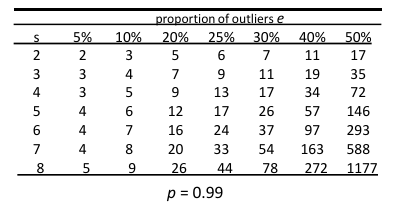
\includegraphics[width=0.6\textwidth]{img/RANSAC_iterations.png}
        \caption{Número de iteraciones necesarias para probabilidad de éxito del 99\% en RANSAC, dependiendo del número de puntos mínimos $s$ y el ratio de outliers $e$.}
        \label{fig:RANSAC_iterations}
    \end{figure}

    \item \textbf{Keep best model:} conservar el mejor modelo matemático, que corresponde a aquel que logró reclutar el \textbf{mayor número de inliers}.
    \item \textbf{Refinement:} opcionalmente, reajustar el modelo final mediante mínimos cuadrados utilizando el conjunto completo de todos los inliers descubiertos. Esto se refiere a recalcular un modelo nuevo usando todos los inliers (del modelo ganador) y sus errores para obtener una estimación más precisa, usando técnicas de optimización global, como \tbf{Mínimos Cuadrados (Least Squares)}. \\
    
    \noindent
    En este nuevo modelo, se obvian las 4 primeras parejas aletorias (el modelo se genera gracias a todos los inliers) y se eliminan los outliers que no se consiguieron juntar, para que no afecten a la precisión del modelo final.
\end{enumerate}

\begin{observacion}
    Puede ocurrir que en las parejas asociadas en el feature matching, haya outliers, de manera que en el algoritmo RANSAC, el modelo usado siempre este comparando la proyección de un keypoint con un matching erróneo, pero eso no es un gran problema, porque el modelo correcto (que se genera a partir de un subconjunto de inliers) seguirá reclutando más inliers que cualquier modelo erróneo generado a partir de outliers, por lo que al final el modelo correcto será el que tenga más votos (inliers) y ganará la competición.\\
\end{observacion}

\section{Aplicaciones de las Características Locales}
Dominar este flujo de descriptores, detectores y RANSAC nos permite habilitar las siguientes tecnologías fundamentales expuestas en las diapositivas:
\begin{enumerate}
    \item \textbf{Image Stitching / Panorama Creation:} unir múltiples fotografías de un paisaje buscando esquinas comunes, emparejando sus descriptores, calculando la homografía con RANSAC y proyectándolas en un lienzo común sin costuras visibles.
    \item \textbf{Reconocimiento de Objetos (Object Recognition):} identificar un objeto en una escena desordenada emparejando sus puntos de interés locales con los de una base de datos del objeto plantilla.
    \item \textbf{Structure from Motion (SfM):} reconstruir la geometría tridimensional 3D de una escena y las posiciones de las cámaras en movimiento rastreando las trayectorias de los puntos de interés emparejados a lo largo de una secuencia de video o colección de imágenes.
\end{enumerate}

